\documentclass[12pt]{article}
\usepackage{latexsym,amssymb,amsmath} % for \Box, \mathbb, split, etc.
% \usepackage[]{showkeys} % shows label names
\usepackage{cite} % sorts citation numbers appropriately
\usepackage{path}
\usepackage{url}
\usepackage{verbatim}
\usepackage{graphicx}
\usepackage{array}
\usepackage{multirow}

% horizontal margins: 1.0 + 6.5 + 1.0 = 8.5
\setlength{\oddsidemargin}{0.0in}
\setlength{\textwidth}{6.5in}
% vertical margins: 1.0 + 9.0 + 1.0 = 11.0
\setlength{\topmargin}{0.0in}
\setlength{\headheight}{12pt}
\setlength{\headsep}{13pt}
\setlength{\textheight}{625pt}
\setlength{\footskip}{24pt}

\renewcommand{\textfraction}{0.10}
\renewcommand{\topfraction}{0.85}
\renewcommand{\bottomfraction}{0.85}
\renewcommand{\floatpagefraction}{0.90}
\usepackage{graphicx}
\usepackage{wrapfig}
\usepackage{lscape}
\usepackage{rotating}
\usepackage{epstopdf}
\makeatletter
\setlength{\arraycolsep}{2\p@} % make spaces around "=" in eqnarray smaller
\makeatother

% change equation, table, figure numbers to be counted inside a section:
\numberwithin{equation}{section}
\numberwithin{table}{section}
\numberwithin{figure}{section}

% begin of personal macros
\newcommand{\half}{{\textstyle \frac{1}{2}}}
\newcommand{\eps}{\varepsilon}
\newcommand{\myth}{\vartheta}
\newcommand{\myphi}{\varphi}
\usepackage[utf8]{inputenc}

% Default fixed font does not support bold face
\DeclareFixedFont{\ttb}{T1}{txtt}{bx}{n}{8} % for bold
\DeclareFixedFont{\ttm}{T1}{txtt}{m}{n}{8}  % for normal

% Custom colors
\usepackage{color}
\definecolor{deepblue}{rgb}{0,0,0.5}
\definecolor{deepred}{rgb}{0.6,0,0}
\definecolor{deepgreen}{rgb}{0,0.5,0}
\definecolor{backcolour}{rgb}{0.96,0.96,0.96}

\usepackage{listings}

% cpp style for highlighting
\newcommand\cppstyle{\lstset{
		language=C++,
        basicstyle=\tiny\ttfamily,
		keywordstyle=\color{blue}\ttfamily,
		stringstyle=\color{red}\ttfamily,
		commentstyle=\color{green}\ttfamily,
		morecomment=[l][\color{magenta}]{\#},
		frame=tb,                         % Any extra options here
showstringspaces=false,            % 
backgroundcolor=\color{backcolour}
}}


% cpp environment
\lstnewenvironment{cpp}[1][]
{
	\cppstyle
	\lstset{#1}
}
{}

% cpp for external files
\newcommand\cppexternal[2][]{{
		\cppstyle
		\lstinputlisting[#1]{#2}}}

% cpp for inline
\newcommand\cppinline[1]{{\cppstyle\lstinline!#1!}}

\newcommand{\IN}{\mathbb{N}}
\newcommand{\IZ}{\mathbb{Z}}
\newcommand{\IQ}{\mathbb{Q}}
\newcommand{\IR}{\mathbb{R}}
\newcommand{\IC}{\mathbb{C}}
\newcommand{\Real}[1]{\mathrm{Re}\left({#1}\right)}
\newcommand{\Imag}[1]{\mathrm{Im}\left({#1}\right)}
\usepackage{booktabs}
\usepackage{caption}
\usepackage{float}
\usepackage{titlesec}
\usepackage{capt-of}
%dashed line
\usepackage{array}
\usepackage{arydshln}
\setlength\dashlinedash{0.2pt}
\setlength\dashlinegap{1.5pt}
\setlength\arrayrulewidth{0.3pt}

%Widows & Orphans & Penalties

\widowpenalty500
\clubpenalty500
\clubpenalty=9996
\exhyphenpenalty=50 %for line-breaking at an explicit hyphen
\brokenpenalty=4991
\predisplaypenalty=10000
\postdisplaypenalty=1549
\displaywidowpenalty=1602
\floatingpenalty = 20000
\usepackage[T1]{fontenc}
\usepackage{fontspec}
\setmainfont[Scale=0.85, Ligatures={Required,Common,Contextual,TeX}]{TeX Gyre Schola} % Incredible font inside latex


\newcommand{\norm}[2]{\|{#1}\|_{{}_{#2}}}
\newcommand{\abs}[1]{\left|{#1}\right|}
\newcommand{\ip}[2]{\left\langle {#1}, {#2} \right\rangle}
\newcommand{\der}[2]{\frac{\partial {#1}}{\partial {#2}}}
\newcommand{\dder}[2]{\frac{\partial^2 {#1}}{\partial {#2}^2}}
\usepackage{enumitem}
\newcommand{\nn}{\mathbf{n}}
\newcommand{\xx}{\mathbf{x}}
\newcommand{\uu}{\mathbf{u}}
\usepackage{tikz}
\usetikzlibrary{arrows}
\usetikzlibrary{positioning}
\usepackage{titlesec}
\newcommand{\junk}[1]{{}}
\usepackage{sectsty}
\usepackage{xcolor}

\newcommand\MyBox[2]{
	\fbox{\lower0.75cm
		\vbox to 1.7cm{\vfil
			\hbox to 1.7cm{\hfil\parbox{1.4cm}{#1\\#2}\hfil}
			\vfil}%
	}%
}

\makeatletter
\renewcommand*\env@matrix[1][\arraystretch]{%
	\edef\arraystretch{#1}%
	\hskip -\arraycolsep
	\let\@ifnextchar\new@ifnextchar
	\array{*\c@MaxMatrixCols c}}
\makeatother

\makeatletter
\renewcommand*\env@matrix[1][*\c@MaxMatrixCols c]{%
	\hskip -\arraycolsep
	\let\@ifnextchar\new@ifnextchar
	\array{#1}}
\makeatother

\definecolor{darkblue}{rgb}{0,0,0.4}
\usepackage[colorlinks = true,
linkcolor = darkblue,
urlcolor  = darkblue,
citecolor = darkblue,
anchorcolor = darkblue]{hyperref}
% set two lengths for the includegraphics commands used to import the plots:
\newlength{\fwtwo} \setlength{\fwtwo}{0.45\textwidth}
% end of personal macros

\begin{document}
\DeclareGraphicsExtensions{.jpg}

\begin{center}
\textsc{\Huge Multi-core Programming} \\[2pt]
	\textsc{\Large Assignment 3}\\
	\vspace{0.5cm}
  Ali Gholami \\[6pt]
  Department of Computer Engineering \& Information Technology\\
  Amirkabir University of Technology  \\[6pt]
  \def\UrlFont{\em}
  \url{https://aligholamee.github.io}\\
\href{mailto:aligholami7596@gmail.com}{\textit{aligholami7596@gmail.com}}
\end{center}

\begin{abstract}
One common example of parallel processing is the implementation of the merge sort within a parallel processing environment. In the fully parallel model, you repeatedly split the sublists down to the point where you have single-element lists. You then merge these in parallel back up the processing tree until you obtain the fully merged list at the top of the tree. In this report, we'll analyze the possibility of Merge-sort parallelization using OpenMP tasks and sections.
\end{abstract} 

\subparagraph{Keywords.} \textit{Merge-sort, Parallel Recursive Sort, Parallel Sort, Heterogeneous Programming, OpenMP, C Programming, C++ Programming, Parallelization, Multi-thread Programming.}

\section{Merge-sort Parallelization with Tasks}
\subsection{Problem Specification}
This assignment focuses on the parallel sorting problem using OpenMP. The goal is to improve the speed of array sorting by implementing the parallelization in recursive section of the sorting algorithm. We'll conduct the two features of OpenMP called \textit{Tasks} and \textit{Sections} respectively. The initial code implemented for the Merge-sort is given below.
\begin{cpp}
		void mergeSort(int *a, int n) {
			int m;
			if (n < 2)
			return;
			m = n / 2;
			mergeSort(a, m);
			mergeSort(a + m, n - m);
			merge(a, n, m);
		}
\end{cpp}

\subsection{Task Parallelization}
Considering the \textit{Tasks} as units of work, we'll generate them by a single thread. These generated tasks are put into a \textit{Task Queue}. The other threads are waiting for the first task to be available. Each thread takes a task from the queue and starts working on it. This idea is clearly described in the figure 1.1 which is brought from the official slides from Intel.
\subsection{Task Execution}
Tasks are queued and executed whenever possible at the so-called task scheduling points. Under some conditions, the runtime could be allowed to move task between threads, even in the mid of their lifetime. Such tasks are called untied and an untied task might start executing in one thread, then at some scheduling point it might be migrated by the runtime to another thread {\UrlFont[by Hristo Iliev on Stackoverflow]}.

\begin{figure}[!h]\centering
	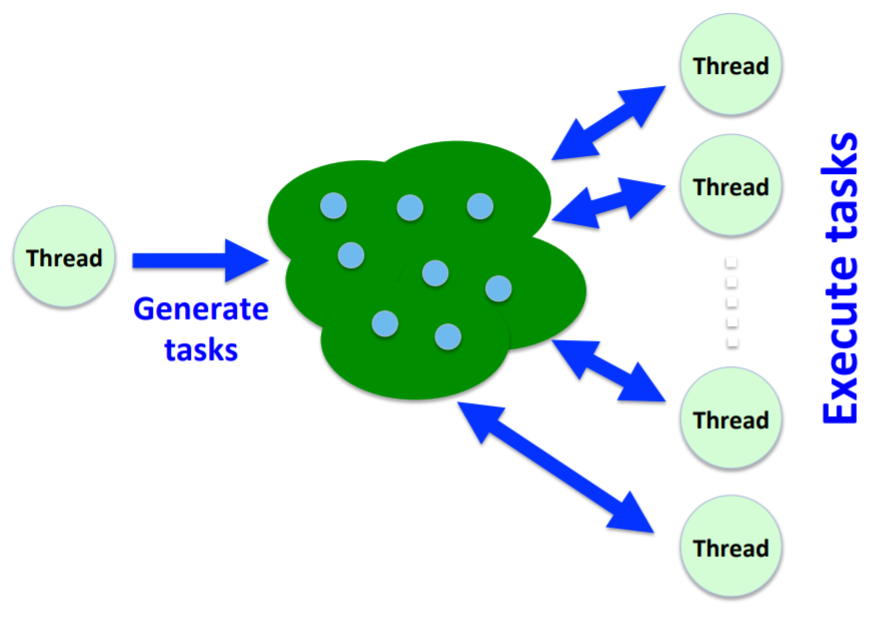
\includegraphics[width=0.7\textwidth]{task_concept.png}
	\caption{Illustration of Task Concept in OpenMP.}
	\label{figsolplot}
\end{figure}

\subsection{Task Parallelization in Recursive Loops}
Tasks are useful in many scenarios as well as recursive loops. In a high-dimensional space, the Merge-sort algorithm generate large numbers of single numbers at the leaves of the computational tree. These leaves can be merged by different threads. Thus, Parallelization can be done in every depth of the tree. An important criteria that needs to be satisfied is that \textit{depths of the tree are dependent on each other}. Thus, when some threads complete their job on some leaves, they have to wait until other threads are done with other leaves. This can be achieved using the \textit{taskwait} directive.

\subsection{Parallelized Recursive Loop}
Here is the final parallelized code for th recursive loops we just talked about. Note that the \textit{parallel region} is implemented \textbf{outside} of the recursive function.
\begin{cpp}
		void mergeSort(int *a, int n) {
			
			int m;
			if(n < 2)
			return;
			
			// else...
			m = n / 2;
			
			#pragma omp task
			mergeSort(a, m);
			
			#pragma omp task
			mergeSort(a + m, n - m);
			
			#pragma omp taskwait
			merge(a, n, m);
		}
\end{cpp}

\subsection{Testing \& Evaluation}
Assuming each \textit{integer} as 4 bytes, we'll be filling the table 1.1 using the average time  computed after 6 times of running the program. According to this assumption, each dimension can be computed as below:
\begin{itemize}
	\item \textbf{100 MB}:  $d = \frac{10^8}{4} = 25 * 10^6$
	\item \textbf{200 MB}:  $d = \frac{2 * 10^8}{4} = 50 * 10^6$
	\item \textbf{300 MB}:  $d = \frac{3 * 10^8}{4} = 75 * 10^6$
	\item \textbf{500 MB}:  $d = \frac{5 * 10^8}{4} = 125 * 10^6$
\end{itemize}

\def\arraystretch{1.3}
\begin{table}[!h]
		\centering
\begin{tabular}{ |p{3cm}||p{2cm}|p{2cm}|p{2cm}|p{2cm}|p{1.5cm}|  }
	
	\hline
	\multicolumn{6}{|c|}{Total Array Size} \\
	\hline
	 Num of Threads & 100 MB & 200 MB & 300 MB & 500 MB & Average Speedup\\
	\hline
		1   & 6.120653    & 12.599889 & 19.009687  &   31.613370 &   -\\
		2   & 8.140178    & 16.292684 & 24.851261  &   41.500230 &   0.85\\
		4   & 4.665155    & 9.426776  & 14.257916  &   23.927245 &   1.9\\
		8   & 3.540851    & 7.224303  & 10.782175  &   19.272577 & 1.2\\
	\hline
\end{tabular}
	\caption{Results of Recursive Loop Parallelization using Tasks.}
\label{figsolplot}
\end{table}

\section{Merge-sort Parallelization with Sections}
Sections are very similar to the tasks in the concept point of view. Unfortunately, sections are not efficient compared to the tasks. The main reason is related to the \textit{time frame} they execute the code.
\subsubsection{The Problem with Sections Block}
Here is a simple but great explanation of the \textit{Sections} bottleneck. Assume we have $n$ threads to run the code ($n > 2$) and there are only $2$ sections defined by the developer. Only $2$ threads start executing the code in each of the \textit{section} block and the other $n-2$ threads should wait at the end of the \textit{sections} parallel block. Recall that the \textit{sections} parallel block contains an \textit{implicit} barrier(shown with *) at the end. Here is the illustration of this phenomenon thanks to the \textit{Hristo Iliev} explanation on the \textit{Stack-overflow}.
\begin{cpp}
						                 [    sections     ]
						Thread 0: -------< section 1 >---->*------
						Thread 1: -------< section 2      >*------
						Thread 2: ------------------------>*------
						...                                *
						Thread N-1: ---------------------->*------
\end{cpp}

\subsection{Parallelized Recursive Loop}
Here is the final parallelized code for the recursive loops using \textit{sections}.
\begin{cpp}
		void mergeSort(int *a, int n) {
			
			int m;
			if(n < 2)
			return;
			
			// else...
			m = n / 2;
			
			#pragma omp parallel sections
			{
				
				#pragma omp section
				mergeSort(a, m);
				
				#pragma omp section
				mergeSort(a + m, n - m);
			}
			merge(a, n, m);
		}
\end{cpp}

\subsection{Testing \& Evaluation}
Assuming each \textit{integer} as 4 bytes, we'll be filling the table 1.1 using the average time  computed after 6 times of running the program. According to this assumption, each dimension can be computed as below:
\begin{itemize}
	\item \textbf{100 MB}:  $d = \frac{10^8}{4} = 25 * 10^6$
	\item \textbf{200 MB}:  $d = \frac{2 * 10^8}{4} = 50 * 10^6$
	\item \textbf{300 MB}:  $d = \frac{3 * 10^8}{4} = 75 * 10^6$
	\item \textbf{500 MB}:  $d = \frac{5 * 10^8}{4} = 125 * 10^6$
\end{itemize}

\def\arraystretch{1.3}
\begin{table}[!h]
	\centering
	\begin{tabular}{ |p{3cm}||p{2cm}|p{2cm}|p{2cm}|p{2cm}|p{1.5cm}|  }
		
		\hline
		\multicolumn{6}{|c|}{Total Array Size} \\
		\hline
		Num of Threads & 100 MB & 200 MB & 300 MB & 500 MB & Average Speedup\\
		\hline
		1   & 6.639830    & 13.757173 & 20.468429  &   34.843211 &   -\\
		2   & 3.523107    & 7.219967  & 10.830306  &   18.208799 &   1.8\\
		4   & 3.519742    & 7.189632  & 10.897979  &   18.089861 &   1\\
		8   & 3.590844    & 7.235916  & 10.896604  &  18.313119  &  1\\
		\hline
	\end{tabular}
	\caption{Results of Recursive Loop Parallelization using Sections.}
	\label{figsolplot}
\end{table}

\section{System Specifications} 
Please refer to {\UrlFont\href{https://www.dropbox.com/s/chkpoyd5rhhf7z8/ASUS_N56JK.html?dl=0}{this}} link to see the complete system specification. These information are extracted using \textit{CPU-Z}.

\end{document}